\documentclass[12pt,a4paper]{article}
\usepackage{datetime}
\usepackage[T1]{fontenc}
\usepackage[utf8]{inputenc}
\usepackage{graphicx} 
\usepackage{url}
\graphicspath{{images/}} 
\renewcommand{\figurename}{Şekil}
\usepackage{geometry}
\usepackage{hyperref}
\usepackage{subcaption}
\usepackage{amsmath}

\title{\bf\fontsize{12pt}{14pt}\selectfont KÜTAHYA SAĞLIK BİLİMLERİ ÜNİVERSİTESİ \\ MÜHENDİSLİK VE DOĞA BİLİMLERİ FAKÜLTESİ}
\date{}
\begin{document}
	
	\maketitle
	\begin{center}
			
\includegraphics[width=0.25\linewidth]{ksbu.png}
	\end{center}
             
	        
	\begin{center}
		\vspace{1cm} 
	\end{center}
	\begin{center}
	\title{\bf\fontsize{12pt}{14pt}\selectfont YAPAY ZEKA DERSİ }
	\end{center}
		\begin{center}
		\title{\bf\fontsize{12pt}{14pt}\selectfont Recurrent Neural Networks(RNN) Kullanarak Hava Durumu Tahmini}
	\end{center}
	\begin{center}
	\vspace{1cm} % Vertical space of 1cm
	\end{center}
	\begin{center}
		
	
	\author{\bf\fontsize{12pt}{14pt}Yusuf KIZILGEDİK \hspace{1.5cm}2118121003}
	
	\begin{center}
	\vspace{1cm} 
	\end{center}
	\date{\textbf{\today}}
	\end{center}
\newpage
 \begin{abstract}
Bu çalışmada, hava durumu tahmininde kullanılan yapay zeka teknikleri ve özellikle tekrarlayan sinir ağlarının (RNN) rolü üzerinde durulmuştur. Çalışmanın amacı, geçmiş hava durumu verilerini kullanarak gelecekteki hava durumunu tahmin etmek için RNN tabanlı bir yapay zeka uygulaması geliştirmektir. Hava durumu tahmini için RNN'nin neden tercih edildiği, kullanılan algoritmalar ve uygulama performansı detaylı bir şekilde açıklanmıştır. Elde edilen sonuçlar, bu uygulamanın hava durumu tahmininde başarılı olduğunu göstermiştir. Ayrıca, diğer algoritmalarla yapılan karşılaştırmalar da değerlendirilmiştir.
\end{abstract}

{\bf\fontsize{12pt}{14pt}\selectfont Anahtar kelimeler:}
Yapay Zeka,RNN,LSTM,Hava Durumu Tahmini, Keras
  \newpage
	\begin{enumerate}

	\item {\bf\fontsize{12pt}{14pt}\selectfont Giriş}\newline\newline
Bu çalışma, hava durumu tahmini için yapay zeka ve özellikle tekrarlayan sinir ağlarının kullanımını incelemektedir. Hava durumu tahmini, zamansal verilerin analizi gerektiren karmaşık bir alandır. Tekrarlayan sinir ağlarının, zamansal ilişkileri daha iyi anlamak için kullanılabilecek çeşitli türleri vardır. Hava durumu tahmini konusunda RNN'nin avantajları ve bu çalışmanın neyi başarmayı hedeflediği burada açıklanmaktadır.

Bu çalışmada, hava durumu tahmininde yapay zeka uygulamalarının önemine dair önceden yapılan çalışmalar ve bu çalışmanın neden önemli olduğu da vurgulanmaktadır. Önceki çalışmalardaki eksiklikler ve bu çalışmanın çözmeyi hedeflediği problemler üzerinde durulmaktadır. Bu çalışmanın amacı, hava durumu tahmininde derin öğrenme tekniklerini kullanarak daha doğru tahminler elde etmektir.

    

\item  {\bf\fontsize{12pt}{14pt}\selectfont Literatür Araştırması}\newline\newline
\begin{itemize}
\item  Weather Prediction Using Recurrent Neural Networks
Bu çalışmada, RNN'lerin sıcaklık, nem, rüzgar hızı gibi hava durumu özelliklerini tahmin etmedeki etkinliği araştırılmıştır. Yazarlar, RNN modellerinin özellikle zamansal verilerdeki bağımlılıkları yakalamada başarılı olduğunu ve bu nedenle hava durumu tahmini için uygun olduğunu vurgulamaktadır. RNN'ler, ardışık veriler arasındaki bağımlılıkları modelleyerek tahmin doğruluğunu artırabilirler\cite{L1}.

\item Long Short-Term Memory Recurrent Neural Network for Weather Prediction
Bu çalışmada, hava durumu tahmini için LSTM (Long Short-Term Memory) adı verilen bir RNN türevi kullanılmıştır. LSTM'ler, uzun vadeli bağımlılık sorununu çözme yeteneğine sahiptir ve bu nedenle daha doğru tahminler yapabilir. Yazarlar, LSTM modellerinin sıcaklık, nem ve rüzgar hızı gibi parametrelerde daha düşük hata oranları gösterdiğini belirtmiştir. LSTM'ler, özellikle eksik verilerin doldurulması ve verilerin normalizasyonu gibi ön işleme teknikleriyle birleştiğinde yüksek performans sergiler\cite{L2}.

\item Forecasting Weather with Recurrent Neural Networks
Bu araştırmada, RNN'lerin hava durumu tahmini için kullanılmasıyla ilgili bir derleme sunulmuştur. Farklı RNN mimarilerinin hava durumu tahmini üzerindeki etkileri incelenmiş ve gelecekteki çalışmalar için önerilerde bulunulmuştur. Çalışma, LSTM ve GRU (Gated Recurrent Unit) gibi farklı RNN türlerinin performansını karşılaştırmış ve her birinin avantajlarını ve dezavantajlarını analiz etmiştir. Ayrıca, mevsimsel ve kısa vadeli tahminlerde bu modellerin nasıl uygulanabileceği tartışılmıştır\cite{L3}.
\end{itemize}


\item  {\bf\fontsize{12pt}{14pt}\selectfont Proje Yaklaşımı}\newline\newline
\begin{itemize}
\item Veri Toplama: İlk adım, hava durumu verilerini toplamak olacaktır. Bu veriler, tarih, saat, sıcaklık, nem, rüzgar hızı, basınç gibi hava koşullarını içermelidir. Hava durumu verileri, kamu hizmeti sağlayıcılarından veya çeşitli hava durumu istasyonlarından alınabilir.

\item Veri Ön İşleme: Toplanan verilerin doğruluğunu ve tutarlılığını sağlamak için ön işleme adımları uygulanmalıdır. Bu adımlar arasında eksik veya hatalı verilerin işlenmesi, veri normalizasyonu ve özellik mühendisliği yer alabilir.

\item Model Seçimi: Ardından, hava durumu tahmini için bir RNN modeli seçilir. LSTM gibi uzun vadeli bağımlılığı ele alan RNN türevleri sıklıkla tercih edilir. Modelin mimarisi, girdi ve çıktı katmanları, saklı katmanlar ve hiperparametreler bu aşamada belirlenir.

\item Model Eğitimi: Seçilen RNN modeli, toplanan ve önceden işlenen veriler kullanılarak eğitilir. Eğitim aşamasında, modelin hava durumu verilerini doğru bir şekilde tahmin etmesi için girdi-veri çiftleri üzerinde optimize edilir.

\item Model Değerlendirmesi: Eğitilen model, belirli bir test veri kümesi üzerinde değerlendirilir. Modelin doğruluğu, ortalama karesel hata (MSE), ortalama mutlak hata (MAE) gibi performans ölçütleri kullanılarak değerlendirilir.

\item Sonuçların Yorumlanması: Elde edilen sonuçlar analiz edilir ve yorumlanır. Modelin ne kadar başarılı olduğu, hangi hava koşullarını daha iyi tahmin ettiği ve potansiyel iyileştirme alanları gibi konular incelenir.
\end{itemize}
\newpage
  \begin{figure}[h]
  	\caption{GANTT Şeması}
  	\vspace{0.5cm} 
  	\centering
  	 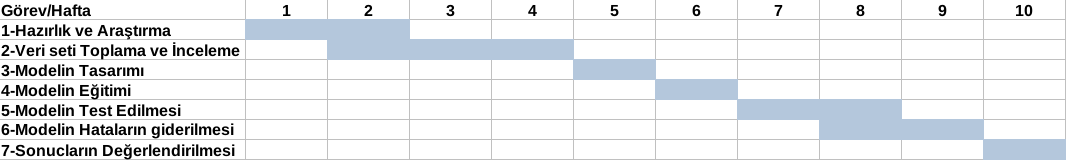
\includegraphics[width=\textwidth,height=\textheight,keepaspectratio]{GanttS.png }
  	
  		\vspace{0.7cm}
  	
  \end{figure}
  \begin{itemize}
         
      \item 
      {\bf\fontsize{12pt}{14pt}\selectfont Hazırlık ve Araştırma:} 
      RNN'ler hakkında temel bilgi edinme ve araştırma yapma, RNN'lerin gerçek hayattaki uygulamalarını inceleme,Proje kapsamı ve hedeflerinin netleştirilmesi.
      \item {\bf\fontsize{12pt}{14pt}\selectfont Veri Seti Toplama ve İnceleme:}  
      Hava durumu tahmini için uygun veri setlerini bulma ve toplama, Veri setlerini temizleme, işleme ve ön inceleme yapma\cite{ulasav_hava_durumu}\cite{ulasav_hava_durumu_verileri}.
      \item {\bf\fontsize{12pt}{14pt}\selectfont  Modelin Tasarımı ve Eğitimi:} 
      RNN modelinin mimarisini belirleme ve tasarlama,
Veri setlerini model için uygun formata dönüştürme, Modelin eğitimi için uygun algoritmaları seçme ve uygulama.
      \item {\bf\fontsize{12pt}{14pt}\selectfont  Modelin Test Edilmesi ve Ayarlanması:} 
      Eğitilen modelin performansını değerlendirme ve test etme,Modelin hata analizi yapma ve iyileştirmeler için ayarlamalar yapma, Modelin doğruluğunu artırmak için optimizasyon yöntemlerini uygulama,
      
      \item {\bf\fontsize{12pt}{14pt}\selectfont Sonuçların Değerlendirilmesi ve Raporlama:}  
      Projenin sonuçlarını derleme ve değerlendirme,
Elde edilen sonuçları raporlama ve sunum hazırlama,
Projenin başarıları, sınırlamaları ve gelecekteki çalışmalar için önerileri tartışma.
  \end{itemize}
 \newpage
\item  {\bf\fontsize{12pt}{14pt}\selectfont Neden RNN?}\newline\newline
	Hava durumu tahmini gibi zamansal verilerin analizi için RNN (Recurrent Neural Networks), standart sinir ağlarına kıyasla daha uygun bir seçenek olabilir. Standart sinir ağları, veriler arasındaki ilişkileri analiz etmek için o anki verilere dayanır ve geçmiş verilerin zaman bağlamını göz ardı eder. Örneğin, bir yarış pistindeki iki aracın yarışını ele alalım: birinci görselde kırmızı araç, mavi araca kıyasla oldukça önde ve birincil konumda ilerlemektedir. Ancak, ikinci görselde kırmızı araç hala birinci sıradadır, ancak mavi araçla arasındaki mesafe oldukça azalmıştır. Bu noktada, standart sinir ağları, her iki görseli ayrı ayrı değerlendirir ve kırmızı aracın kazanacağını tahmin eder. Ancak, RNN, geçmiş verilerin zaman bağlamını dikkate alarak analiz yapar. Dolayısıyla, ikinci görseldeki durumda, mavi aracın mesafeyi kapatma eğiliminde olduğunu ve sonucun değişebileceğini tahmin eder. Bu nedenle, zaman serileri gibi zamansal verilerle çalışırken RNN, zaman bağlamını dikkate alarak daha doğru tahminlerde bulunabilir\cite{deep_learning_turkiye}. \newline\newline
 \begin{figure}[htbp]
    \centering
    \begin{subfigure}[b]{0.45\textwidth}
        \centering
        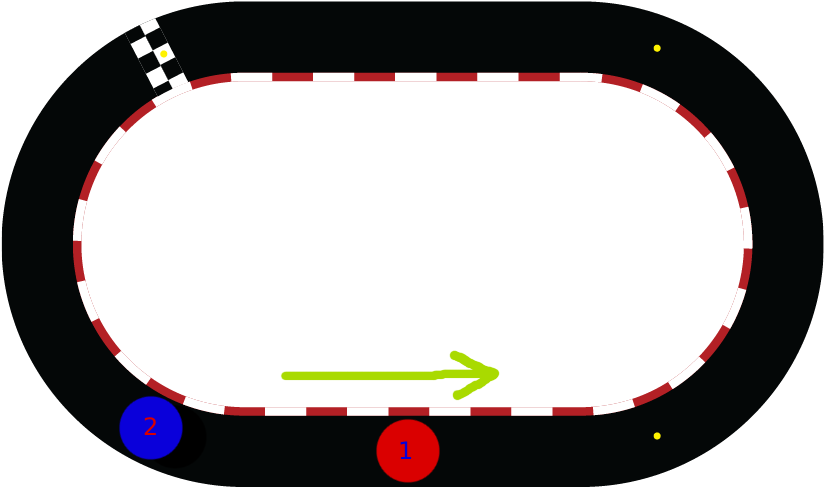
\includegraphics[width=\textwidth]{pist alanı.png}
        \caption{1.Göresel}
        \label{fig:resim1}
    \end{subfigure}
    \hfill
    \begin{subfigure}[b]{0.45\textwidth}
        \centering
        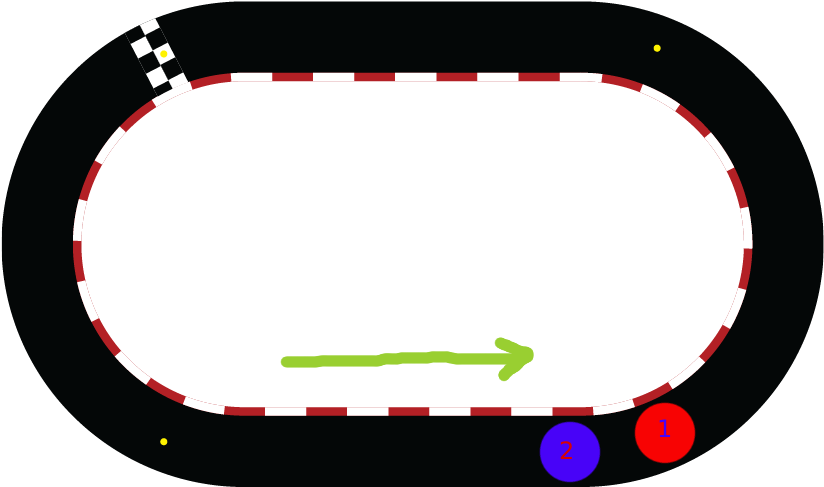
\includegraphics[width=\textwidth]{yarıspisti2.png}
         \caption{2.Görsel}
        \label{fig:resim2}
    \end{subfigure}
    
    \label{fig:yan_yana_resimler}
\end{figure}
 \newpage
 \item  {\bf\fontsize{12pt}{14pt}\selectfont RNN Türleri}\newline
 \begin{itemize}
     \item {\bf\fontsize{12pt}{14pt}\selectfont Vanilla RNN (Temel RNN):}   Basitçe geçmiş zaman adımlarını dikkate alarak bir sonraki adımın tahminini yapar. Ancak, zamanla kaybolan (vanishing gradients) sorunu nedeniyle uzun vadeli bağlantıları yakalamakta zorlanabilir.
     \item {\bf\fontsize{12pt}{14pt}\selectfont Long Short-Term Memory (LSTM):} LSTM, zaman serisi verilerinde uzun vadeli bağımlılıkları daha etkili bir şekilde modellemek için tasarlanmıştır. Hava durumu tahmini gibi zaman serisi problemleri için çok kullanışlıdır.
     \item {\bf\fontsize{12pt}{14pt}\selectfont Gated Recurrent Unit (GRU):} GRU, LSTM'e benzer şekilde uzun vadeli bağımlılıkları ele almak için tasarlanmıştır. Ancak, LSTM'e kıyasla daha az parametreye sahiptir, bu da eğitim sürecini hızlandırabilir.
     \item {\bf\fontsize{12pt}{14pt}\selectfont Bidirectional RNN (BRNN):} BRNN, geçmiş ve gelecek zaman adımlarını ayrı ağlarda işleyerek, her bir zaman adımında hem önceki hem de sonraki verileri dikkate alır. Bu şekilde, mevcut zamandaki tahminler için daha kapsamlı bir bağlam sağlar.
     \item {\bf\fontsize{12pt}{14pt}\selectfont Deep RNN:} Birden fazla katmana (layer) sahip RNN'lerdir. Daha derin yapılar, daha karmaşık zaman serisi ilişkilerini yakalamak için kullanılabilir.
     \item {\bf\fontsize{12pt}{14pt}\selectfont CNN-RNN Hibrit Modeller:} Bazı durumlarda, zaman serisi verilerini işlemek için Convolutional Neural Networks (CNN) ile RNN'leri birleştiren modeller de etkilidir. Özellikle uzaysal yapıyı (örneğin, hava durumu haritaları) dikkate almak istediğinizde, bu tür hibrit modeller kullanışlı olabilir.\newpage
    Hava durumu tahmini gibi zaman serisi problemlerinde sık kullanılan iki RNN türü LSTM ve GRU'dur. Kendi projemde hangisini kullanacağıma karar vermek amacıyla, koduma ikisini de entegre edip sonuçları karşılaştıracağım. Bu karşılaştırmaya göre hangisini kullanacağıma karar vereceğim.
 \end{itemize}
 \item {\bf\fontsize{12pt}{14pt}\selectfont LSTM}\newline\newline
Uzun Kısa-Term Hafıza (LSTM), hava durumu tahmini gibi zaman serisi problemlerinde oldukça etkili olan bir tür Recurrent Neural Network (RNN)’dir. LSTM, sıralı verilerin analizi için kullanılır ve özellikle zaman serileri gibi uzun süreli bağımlılıklar içeren verilerin işlenmesinde etkilidir\cite{lstmnedir}.

\begin{figure}[h]
  	
  	\vspace{0.5cm} 
  	\centering
  	 \includegraphics[width=\textwidth,height=\textheight,keepaspectratio]{lstmyapısı.png }
  	\caption{LSTM yapısı}
  		\vspace{0.7cm}
  	
  \end{figure}
\begin{itemize}
    \item Şekil 3'de, LSTM mimarisin anlatımı kolaylığı icin bir görsel verilmiştir. Görselde 3 adet LSTM hücresi bulunmaktadır. Bu LSTM hücreleri, önceki hücrenin çıktılarını, yani h ve C değerlerini, x girdisi ile birleştirerek yeni h ve C çıktılarını oluşturur. Son LSTM hücresinin çıktısı da  sonucu verir.
\end{itemize}

\begin{figure}[h]
  	
  	\vspace{0.4cm} 
  	\centering
  	 \includegraphics[width=15cm,height=15cm,keepaspectratio]{lstmyapısı2.png }
  	\caption{LSTM\cite{lstmyapısı2}}
  		\vspace{0.4cm}
  	
  \end{figure}
\newpage
\begin{itemize}
    \item LSTM nin doğru gösterimi şekil 4 de verilmiştir.Bu modelimizde aslında bir hücre kendi kendine t zamanında bir girdiyi kullanarak t zamanında c ve h cıktılarını oluşturuyor.C ve H yi bir sonraki adımda kullanmak için kendisiyle paylaşıyor.Böylelikle bir sonraki adımda yeni bir c,h ve yeni bir x girdisiyle calışıyor.
\item Bir LSTM ağı oluşturmanın ilk adımı, gerekli olmayan ve hücreden çıkarılacak olan bilgileri belirlemektir. 
Bu veri tanımlama ve hariç tutma işlemine, \( t-1 \) zamanında son LSTM biriminin (\( h_{t-1} \)) çıktısını ve 
\( t \) zamanında mevcut girdiyi (\( X_t \)) alan sigmoid fonksiyonu karar verir. Ek olarak, sigmoid fonksiyonu eski çıktının hangi kısmının elenmesi gerektiğini belirler. 
Bu kapıya unutma kapısı (veya \( f_t \)) denir\cite{lstmmimarisi}.
\newpage
\item Giriş Kapısı yeni girişten (\( X_t \)) gelen bilgileri kararlaştırır, depolar ve ayrıca hücre durumunu günceller.
Bu adım, sigmoid katman ve ikinci tanh katmanı olmak üzere iki bölümden oluşur.
İlk olarak, sigmoid katmanı, yeni bilginin güncellenip güncellenmeyeceğine (0 veya 1) karar verir ve 
ikinci olarak, tanh fonksiyonu, önem düzeylerine (-1 ile 1 arasında) karar vererek, geçen değerlere ağırlık verir.
Yeni hücre durumunu güncellemek için bu iki değer çarpılır. 
Bu yeni bellek daha sonra eski belleğe (\( C_{t-1} \)) eklenir ve sonuç olarak \( C_t \) elde edilir\cite{lstmmimarisi}.
\item Sigmoid katmanına sahip çıkış kapısı, hücre durumunun hangi kısımlarının çıktıya iletileceğine karar verir.
Ardından, sigmoid kapısından gelen çıktı (\(O_t\)), hücre durumu (\(C_t\)) üzerinden tanh katmanı tarafından oluşturulan yeni değerle çarpılır\cite{lstmmimarisi}.

\begin{figure}[h]
    \centering
    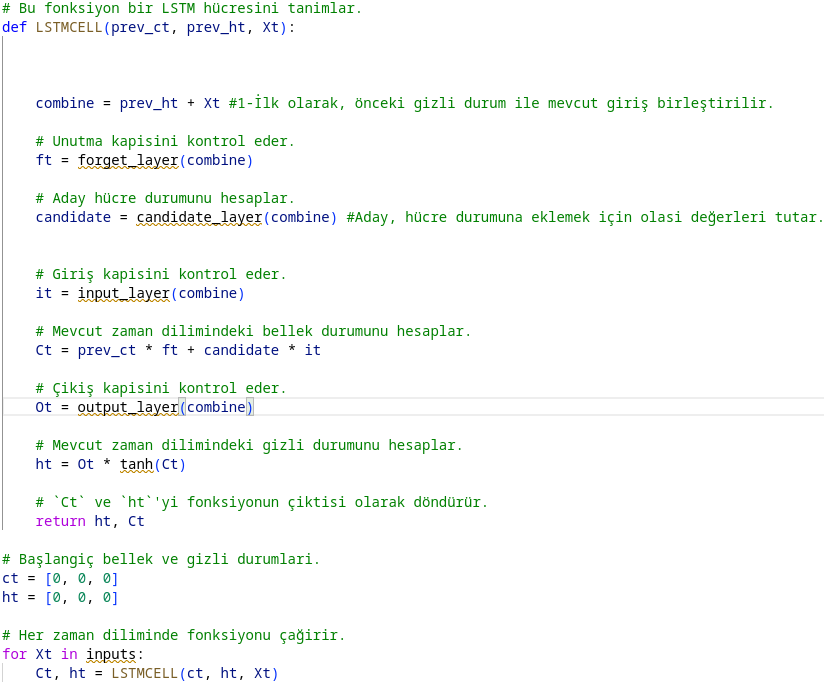
\includegraphics[width=\textwidth,height=\textheight,keepaspectratio]{lstmmimarisikod.png}
    \caption{LSTM python pseudo code \cite{lstmkod} }\label{fig:lstmkod}
\end{figure}
   
\end{itemize}

\item {\bf\fontsize{12pt}{14pt}\selectfont GRU}\newline\newline

GRU modeli, "Gated Recurrent Unit" anlamına gelir ve nöral ağlar içinde popüler bir tür tekrarlayan sinir ağı (RNN) birimidir. GRU, özellikle doğal dil işleme, zaman serisi analizi ve benzeri ardışık veri tabanlı görevlerde kullanılır.GRU, LSTM'nin daha basit ve hesaplama açısından daha verimli bir alternatifi olarak geliştirildi.GRU, LSTM'nin sahip olduğu bazı karmaşık yapıları ve kapıları sadeleştirerek benzer bir performans sunar
    
\begin{figure}[h]
  	
  	\vspace{0.4cm} 
  	\centering
  	 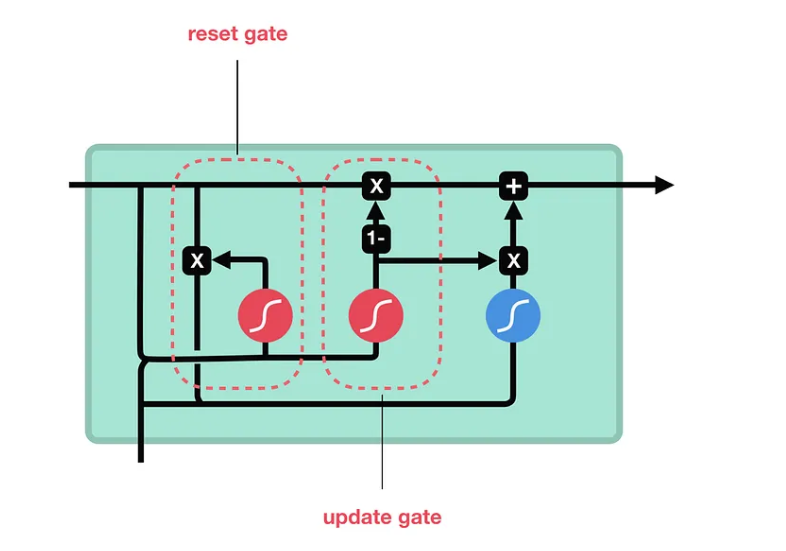
\includegraphics[width=15cm,height=15cm,keepaspectratio]{GRUmimarisi.png }
  	\caption{GRU\cite{GRU}}
  		\vspace{0.4cm}
  	
  \end{figure}
  \par
  {\bf\fontsize{12pt}{14pt} Güncelleme Kapısı:}
Güncelleme kapısı, hücre durumunun ne kadarının bir sonraki durum için korunacağına ve ne kadarının güncelleneceğine karar verir. Güncelleme kapısı değeri, önceki gizli durum ve mevcut girişe bağlı olarak hesaplanır. Bu kapı, hücre durumunun ne kadarının korunacağını kontrol eder.
\newpage
{\bf\fontsize{12pt}{14pt} Reset Kapısı}
  Reset kapısı, hücre içindeki geçmiş bilginin ne kadarının unutulacağına veya sıfırlanacağına karar verir. Reset kapısı da önceki gizli durum ve mevcut girişe bağlı olarak hesaplanır. Bu kapı, eski gizli durumun yeni bilgiye ne ölçüde karışacağını belirler.

\begin{figure}[h]
    \centering
    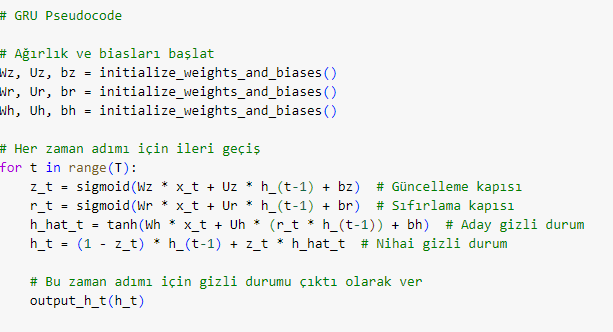
\includegraphics[width=0.9\textwidth,height=0.7\textheight,keepaspectratio]{GRU pseudo kod.png}
    \caption{GRU Kod }
    \label{fig:havadurum}
\end{figure}
\newpage

\par
\item {\bf\fontsize{12pt}{14pt}\selectfont LSTM ve GRU}\newline\newline


\begin{itemize}
    \item GRU, genellikle LSTM'e göre daha hızlı ve hafif çalışır çünkü daha az karmaşıktır.
\item GRU'nun daha düşük bellek tüketimi vardır, bu nedenle veri ve model boyutları arttığında daha iyi çalışabilir.
\item LSTM, karmaşık zaman serisi modellerinde daha iyi genelleme yapabilir, ancak genellikle GRU da benzer performans sergiler.
\item GRU, LSTM'e göre daha basittir. Unutma ve giriş kapıları yerine güncelleme ve sıfırlama kapıları vardır. Bu da daha az parametre ve daha hızlı çalışma anlamına gelir.
\item GRU genellikle daha hızlı ve daha hafif olması nedeniyle tercih edilir, ancak LSTM'nin uzun vadeli bağımlılıkları daha iyi modelleyebilme yeteneği vardır. 

 \newpage
\item{\bf\fontsize{12pt}{14pt}\selectfont Hava Durumu Tahmini Kod} 
\begin{figure}[h]
    \centering
    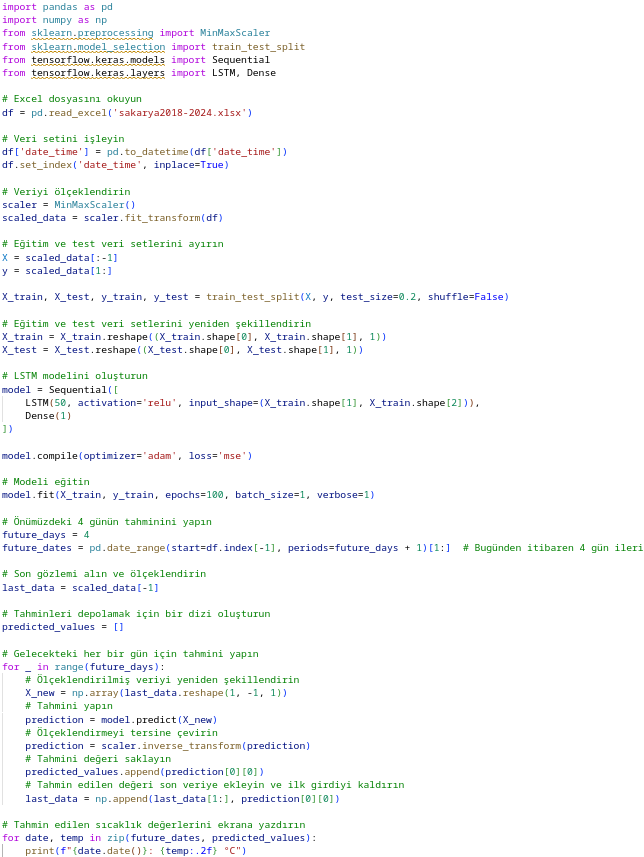
\includegraphics[width=0.9\textwidth,height=0.7\textheight,keepaspectratio]{ilkkod.png}
    \caption{Hava Durumu Tahmini Temel Kod \cite{medium_weather_forecasting}}
    \label{fig:havadurum}
\end{figure}
\begin{itemize}
   

\item 
Yapay sinir ağlarının türlerinden biri olan Uzun Kısa Süreli Bellek (LSTM) modelini kullanan bir Python kodu yazdım. Başlangıçta, bu kod doğru tahminler yapmıyordu ve sonuçlar beklenenin oldukça dışında, tuhaf değerler üretiyordu. Bu durumu düzeltmek ve algoritmanın performansını artırmak için bir dizi iyileştirme yaptım.
\newpage

\begin{figure}[h]
    \centering
    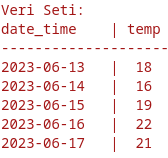
\includegraphics[width=0.9\textwidth,height=0.2\textheight,keepaspectratio]{veriseti.png}
    \caption{Veri Seti}
    
\end{figure}
\item {\bf\fontsize{12pt}{14pt}\selectfont Veri Ön İşleme}   Herhangi bir makine öğrenimi projesinde olduğu gibi, veri ön işleme adımı hava durumu tahmini için de kritiktir. İlk adım olarak, hava durumu veri setimizi alırız. Örneğimizde, hava durumu ölçümleri Sakarya şehrimizin 2018-2024 yılları arasındaki  tarih bilgilerini içeren bir veri seti kullanıyoruz. Veri setimizi Pandas kütüphanesi aracılığıyla yükleriz ve tarih saat sütununu indeks olarak ayarlarız. Daha sonra, veriyi ölçeklendirme işlemine tabi tutarız. Bu, tüm değerleri belirli bir aralığa (genellikle [0, 1] aralığına) yeniden ölçeklendirir ve modelin daha iyi performans göstermesine yardımcı olur\cite{ulasav_hava_durumu}.
\newpage
\begin{figure}[h]
    \centering
    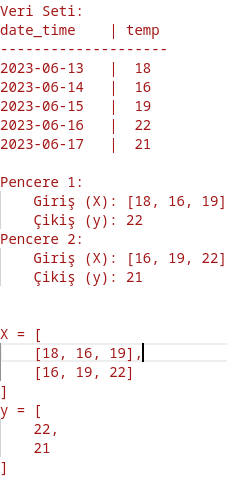
\includegraphics[width=0.9\textwidth,height=0.5\textheight,keepaspectratio]{windowveri1.png}
    \caption{Pencere Veri}
    
\end{figure}
\item {\bf\fontsize{12pt}{14pt}\selectfont Veriyi Window Haline Getirme}   LSTM gibi zaman serisi modelleriyle çalışırken, veriyi pencere (window) haline getirmek yaygın bir uygulamadır. Bu, belirli bir zaman dilimindeki verileri bir araya getirerek, modelin zamansal ilişkileri daha iyi öğrenmesine olanak tanır. Örneğin, son üç günün hava durumu verilerini kullanarak, bir sonraki günün sıcaklık tahminini yapabiliriz. Bu işlem, bir veri penceresi boyunca belirli bir adımda gezinerek gerçekleştirilir.
Yukarıdaki görselde, verinin pencere haline getirilmesini gösteren bir örnek bulunmaktadır. Her adımda, belirli bir pencere boyutu alınır ve bu pencere boyunca sıcaklık verileri toplanır. Bu, X ve y verilerini oluşturur ve modelin eğitimi için kullanılır.
\item {\bf\fontsize{12pt}{14pt}\selectfont Dropout}  Aşırı öğrenmeyi önlemek için yaygın olarak kullanılan bir tekniktir. Bu teknik, rastgele belirlenen bir oranda ağdaki nöronların çıkartılmasını sağlar. Bu, ağın genelleştirme yeteneğini artırır ve aşırı uyumun önüne geçer. Modelimizde Dropout katmanları kullanarak, her eğitim döneminde belirli bir oranda nöronları rastgele devre dışı bırakırız.
\item {\bf\fontsize{12pt}{14pt}\selectfont EarlyStopping}  Modelin eğitimini belirli bir kriter karşılandığında durduran bir geri çağrıdır. Bu, modelin aşırı uyuma meyilli olduğu durumlarda ağın eğitimini zamanında durdurarak, ağın genelleme yeteneğini artırır. Örneğin, modelin kaybı artık azalmıyorsa veya doğrulama kaybı artmaya başlarsa, eğitimi durdurabiliriz.
\item {\bf\fontsize{12pt}{14pt}\selectfont Model Karmaşıklığının Artırılmas} Modelin karmaşıklığını artırmak için daha fazla LSTM katmanı eklendi. LSTM katmanları, zaman serisi verilerindeki karmaşık ilişkileri yakalamak için kullanılır. Modelin karmaşıklığını artırmak, daha fazla öğrenme kapasitesi sağlayabilir ve daha karmaşık veri yapılarını daha iyi modelleyebilir.
\item {\bf\fontsize{12pt}{14pt}\selectfont Daha Fazla Epoch Sayısının Kullanılması} Modelin eğitim sürecinde daha fazla epoch (iterasyon) sayısı kullanıldı. Daha fazla epoch, modelin daha fazla öğrenme fırsatı elde etmesini sağlar. Bu, modelin daha iyi uyum sağlamasını ve daha doğru tahminler üretmesini sağlayabilir.
\newpage
\item {\bf\fontsize{12pt}{14pt}\selectfont MinMAxScaler }\newline\newline
Makine öğrenmesinde, veri ölçekleme önemli bir adımdır.
MinMaxScaler, verileri belirli bir aralığa dönüştürmek için kullanılır, genellikle 0 ile 1 arasına.Bu yöntem, özellikle verilerin belirli bir aralıkta olmasının önemli olduğu durumlarda kullanışlıdır\cite{minmax}.

\[
X_{\text{scaled}} = \frac{X - X_{\min}}{X_{\max} - X_{\min}} \times (\text{max} - \text{min}) + \text{min} \cite{minmax}
\]
\begin{figure}[h]
    \centering
    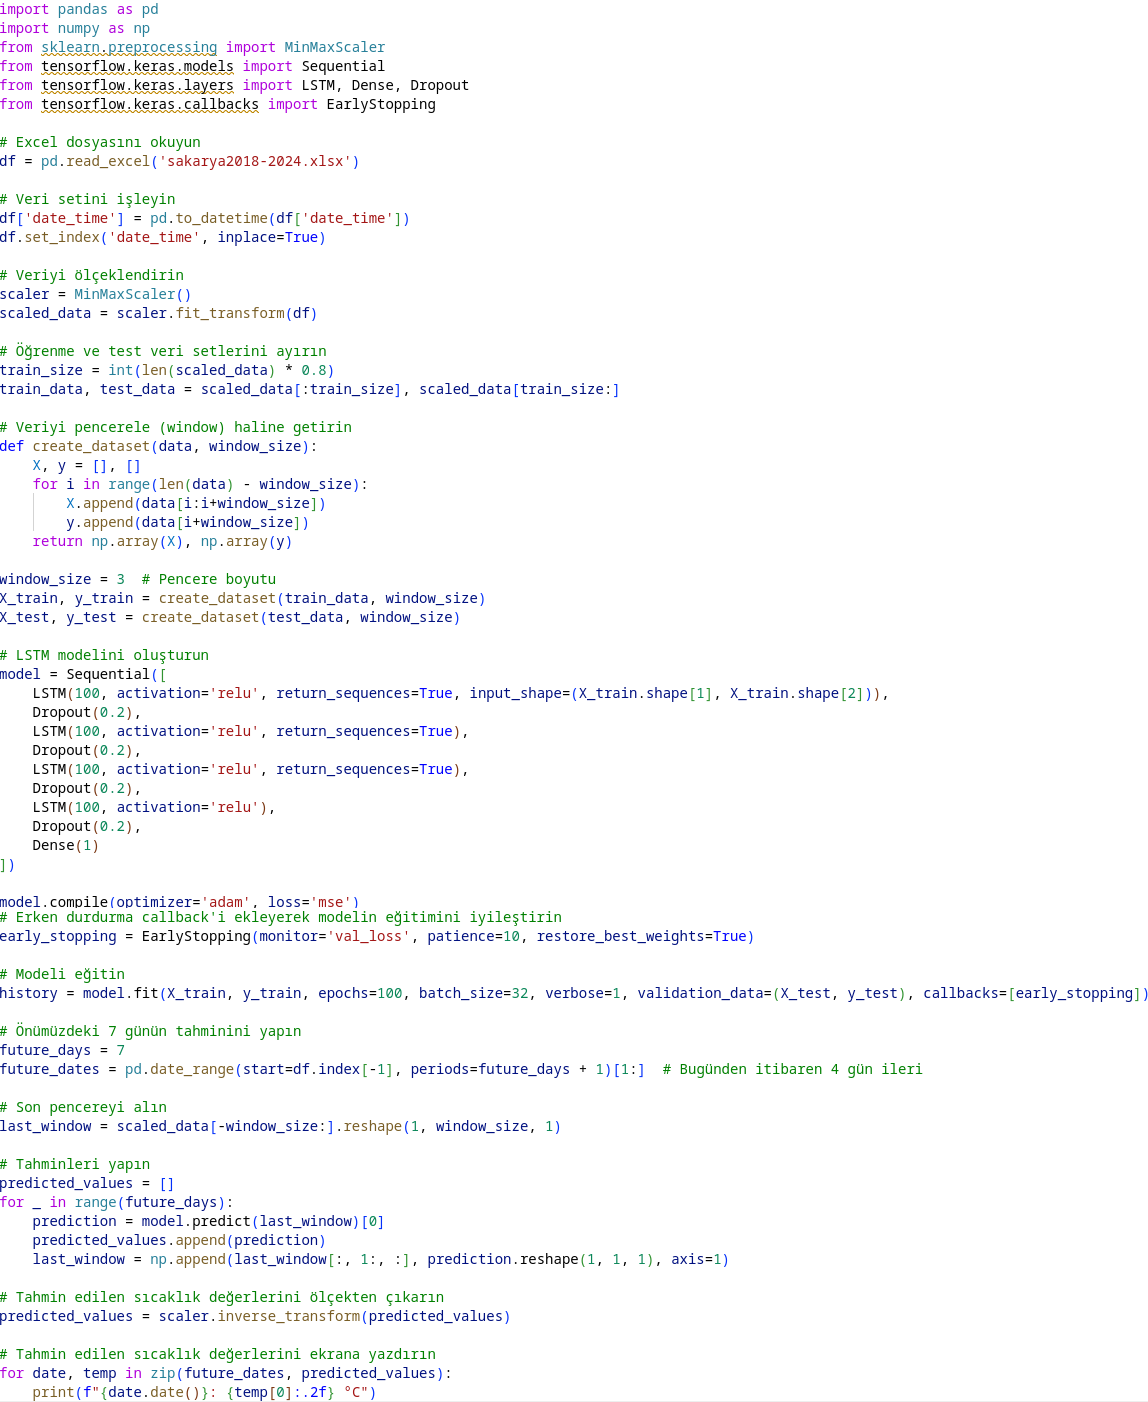
\includegraphics[width=0.9\textwidth,height=0.7\textheight,keepaspectratio]{havadurumtahmini1.png}
    
    \caption{Hava Durumu Tahmini geliştirilmiş Kod \cite{medium_weather_forecasting}}
    \label{fig:havadurum}
\end{figure}
\item Modelde gerçekleştirdiğim iyileştirmelerden sonra, sonuçların ne kadar geliştiğini belirlemek için eski ve yeni sonuçları karşılaştırdım. 



\begin{table}[h!]
\centering
\caption{İyileştirme sonunda çıktı karşılaştırılması}
\begin{tabular}{|c|c|c|c|}
\hline
\textbf{TARİH} & \textbf{Gerçek değer} & \textbf{kod1} & \textbf{kod2} \\
\hline
2023-11-24 & 9    & 8.97      & 8.64 \\
\hline
2023-11-25 & 9    & 565.90    & 9.01 \\
\hline
2023-11-26 & 10   & 27567.37  & 9.44 \\
\hline
2023-11-27 & 2    & 1292014.62 & 9.65 \\
\hline
2023-11-28 & 2    & 60554036.00 & 9.90 \\
\hline
\end{tabular}
\end{table}


Son geliştirmelerimiz sonucunda, modelimizdeki çıktılarda önemli bir doğruluk artışı elde ettik. 



\item LSTM ile GRU karşılaştırmıştık Geliştirdiğimiz bu koda ikisinide entegre edip sonuçlarını karşılaştırdım 

\begin{table}[h!]
\centering
\caption{LSTM ve GRU çıktıları}
\begin{tabular}{|c|c|c|c|}
\hline
\textbf{TARİH} & \textbf{Gerçek değer} & \textbf{GRU} & \textbf{LSTM} \\
\hline
2023-11-24 & 9    & 8.62  & 8.64 \\
\hline
2023-11-25 & 9    & 8.49  & 9.01 \\
\hline
2023-11-26 & 10   & 8.44  & 9.44 \\
\hline
2023-11-27 & 2    & 8.36  & 9.65 \\
\hline
\end{tabular}
\end{table}

\item 
İleriki geliştirmelerimde projemin daha iyi sonuç vermesi için LSTM ile devam etmeye karar verdim.
\end{itemize}
\end{itemize}

  \item {\bf\fontsize{12pt}{14pt}\selectfont RNN ile Küresel Isınma }\newline\newline
  İklimin giderek değişmesi RNN tabanlı hava durum tahmin uygulamasının öngörü yapmasını daha zor hale getirebilir.Bu nedenle , hava durumu tahmin projelerinde küresel ısınmanın etkilerini dikkate almak ve modelleri daha esnek ve uyarlanabilir hale getirmek, tahminlerin doğruluğunu artırmak için kritik öneme sahiptir\cite{mgm_hava_iklim}.

\item {\bf\fontsize{12pt}{14pt}\selectfont Veri Çeşitliliği }\newline\newline
Modelimizin daha iyi bir performans göstermesi için veri çeşitliliğini artırmak istedik ve bu şekilde daha iyi bir sonuç almayı amaçladık. Ancak bunu yaparken, boyut uyumsuzluğundan dolayı bir hatayla karşılaştık ve hatayı çözemeyince tüm veri çeşitlerini hesaplattırdık.

\begin{table}[h]
\centering
\caption{Ortalama Hava Koşulları}
\begin{tabular}{|l|l|l|l|l|l|}
\hline
\textbf{Tarih} & \textbf{Veri Türü} & \textbf{Sıcaklık} & \textbf{Rüzgar Hızı} & \textbf{Rüzgar Yönü} & \textbf{Nem} \\ \hline
2023-11-26 & Gerçek & 6.1 & 2 & 168    & 60 \\ \hline
2023-11-26 & Tahmin & 6.7 & 1.3  & 172 & 60.5\\ \hline
2023-11-27 & Gerçek & 1.2  & 1.5  & 191.5 &51 \\ \hline
2023-11-27 & Tahmin & 8.65 &1.3 & 175 & 57 \\ \hline
2023-11-28 & Gerçek & 5.5 & 1.3 & 150     & 51\\ \hline
2023-11-28 & Tahmin & 6.5 & 1.3 & 172 &61 \\ \hline
2023-11-29 & Gerçek & 9.7 & 1.6 & 145.6     & 64.4 \\ \hline
2023-11-29 & Tahmin &6.6      &1.3      & 170   & 59 \\ \hline

\end{tabular}
\end{table}
\newpage
\item {\bf\fontsize{12pt}{14pt}\selectfont Boyut uyumsuzluğu nedir? }\newline\newline
  Veri analizi veya makine öğrenimi gibi alanlarda, veri işleme adımlarında boyut uyumsuzlukları sıkça karşılaşılan sorunlardan biridir.Bir modelin başarılı bir şekilde çalışabilmesi için, modelin giriş verisiyle çıkış verisi arasında uygun boyut uyumu sağlanmalıdır. Giriş verisi, modelin beklediği şekle (shape) sahip olmalıdır; aynı şekilde, modelin çıkışı da beklenen bir şekilde oluşturulmalıdır. Ancak, giriş ve çıkış boyutları arasında bir uyumsuzluk varsa, modelin doğru şekilde çalışması engellenebilir ve genellikle 'boyut uyumsuzluğu' hatası (shape mismatch error) ile karşılaşılır.

\item {\bf\fontsize{12pt}{14pt}\selectfont Lstm Boyut Uyumsuzluğu }\newline\newline
Modelde giriş ve cıkış verilerinin boyutlarının uymamasından dolayı boyut uyuşmazlığı hatası alındı.
\begin{itemize}
    \item İlk başta, modelin sonuçlarını karşılaştırmak için boyut uyumsuzluğunu gidermeden önce, tüm verilerin tahmin edilmesini istedim. Böylece herhangi bir boyut uyumsuzluğu olmadan sonuçları görebilirdim.
    \item Bu projede sadece sıcaklık değerlerine ihtiyacımız vardı. Bu gereksinimi karşılamak için boyut uyumsuzluğunu çözmek için adımlara başladım.
\item İlk olarak \texttt{model.predict(last\_window)} çağrısından dönen tahminin şekli ve değeri kontrol edildi. Python'un shape özelliği kullanılarak ekrana yazdırıldı.
\begin{figure}[h]
  	
  	\vspace{0.5cm} 
  	\centering
  	 \includegraphics[width=\textwidth,height=\textheight,keepaspectratio]{predict shape .png }
  	\caption{kod}
  		\vspace{0.7cm}
  	
  \end{figure}
\newpage
\item Kodda np.append() işlemi, \texttt{last\_window}'ın sonuna prediction'ı eklemek için kullanılıyor. Zaman birimi olarak son örneği ve tahminlenen değerler arasında bir ilişki olduğundan, tahminlenen değeri \texttt{last\_window}'ın sonundaki bir zaman birimi olarak yerine koyarak hatayı cözme hedeflendi ama yeni bir hata çıktı
\begin{figure}[h]
  	
  	\vspace{0.5cm} 
  	\centering
  	 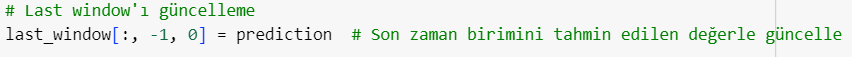
\includegraphics[width=\textwidth,height=\textheight,keepaspectratio]{lastwindow güncelleme.png }
  	\caption{kod}
  		\vspace{0.7cm}
  	
  \end{figure}


\item \texttt{predict(scaler.inverse\_transform())}  işlemi, giriş olarak bir matris bekler, bu nedenle prediction'ın şeklini (1, 1) değil (1, 4) yapmalıyız. Bunun için prediction'ın şeklini değiştirmek gerekti. 

\begin{figure}[h]
  	
  	\vspace{0.5cm} 
  	\centering
  	 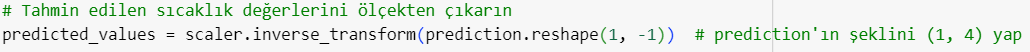
\includegraphics[width=\textwidth,height=\textheight,keepaspectratio]{predictionşekil.png }
  	\caption{kod}
  		\vspace{0.7cm}
  	
  \end{figure}


Bu adımlardan sonra Hata alınmadan istediğimiz değer alındı

\end{itemize}
\newpage
\item {\bf\fontsize{12pt}{14pt}\selectfont Lstm Boyut Uyumsuzluğu Bir Diğer Yöntem }\newline\newline
\begin{itemize}
    


\item İlk başta \texttt{predicted\_values} listesi oluşturuluyor ve her tahmin edilen değer bu listeye ekleniyor. Sonra, \texttt{last\_window} güncellenmeden her tahminden sonra ilerliyoruz. Tüm tahminler toplandıktan sonra, bu değerler geri ölçeklendirilip (\texttt{inverse\_transform}) gerçek dünyadaki değerlere dönüştürülüyor. Ancak, bu işlem sonrasında tahmin edilen sıcaklık değerleri her gün aynı sonucu veriyordu. Bu durumda bir hata olduğunu düşünerek yeni bir yöntem aramaya koyuldum. \texttt{last\_window}'u güncelleme kararı aldım ve sıcaklık değerini alırken bunu uyguladım. Ancak, bu yöntemi uyguladığımda, veri setimdeki diğer veri türlerinin eğitime katkısı olmadığı için veri setimin çeşitliliği bir anlam ifade etmiyordu.
\item Bir diğer yöntem ise tahmin yapılırken sadece sıcaklık (ilk sütun) değerini doldurduk ve diğer sütunları 0 olarak bıraktık.


 \item Veriyi ölceklendirmesinde yeni yöntemde, tahmin edilen sıcaklık değerlerini geri dönüştürmek için scaler.inversetransform() yerine sadece hedef değişkenin minimum ve maksimum değerlerini kullanıyoruz. Bu, işlemi daha basit ve kontrollü hale getiriyor, boyut uyuşmazlıklarını ve hataları önlüyor. Özellikle tek bir değişkeni geri dönüştürmek gerektiğinde, bu yöntem daha esnek ve güvenilir bir çözüm sunuyor.

 \begin{figure}[h]
  	
  	\vspace{0.5cm} 
  	\centering
  	 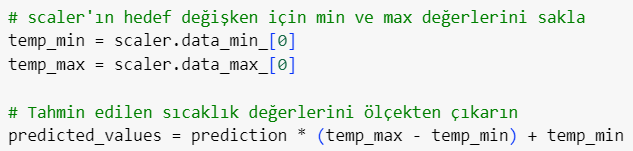
\includegraphics[width=\textwidth,height=\textheight,keepaspectratio]{maxminkod.png}
  	\caption{MAXMİN KOD}
  		\vspace{0.7cm}
  	
  \end{figure}
  \[
X_{\text{scaled}} = \frac{X - X_{\min}}{X_{\max} - X_{\min}} \times (\text{max} - \text{min}) + \text{min} \cite{minmax}
\]

\end{itemize}





\newpage

\item {\bf\fontsize{12pt}{14pt}\selectfont Model Kayıp Grafiği }\newline\newline
  Model kayıp grafiği, modelin eğitim ve doğrulama kayıplarını gösterir.Model kayıp grafiği, modelin eğitim sürecinde nasıl performans gösterdiğini ve aşırı öğrenme (overfitting) veya eksik öğrenme (underfitting) olup olmadığını anlamak için önemlidir. Eğitim kaybının zamanla azaldığı ve doğrulama kaybının nasıl bir eğilim gösterdiği analiz edilir\cite{lgrafik}.
\begin{figure}[h]
  	
  	\vspace{0.5cm} 
  	\centering
  	 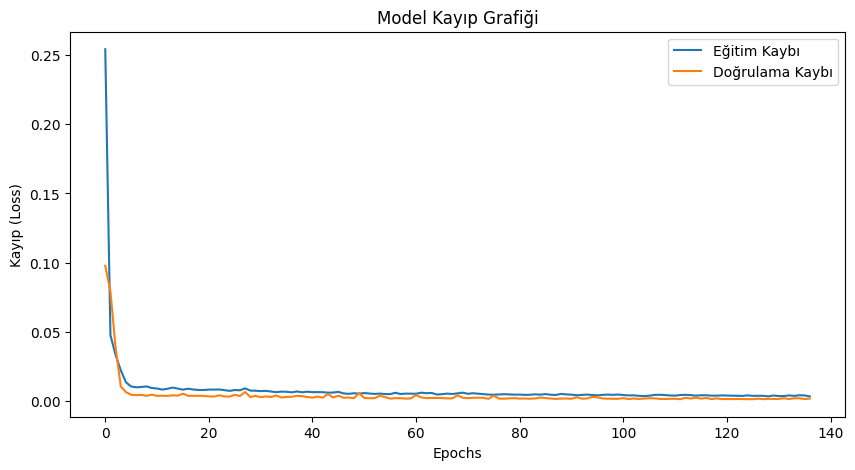
\includegraphics[width=\textwidth,height=\textheight,keepaspectratio]{MkayıpGrafiği.png}
  	\caption{Model Kayıp Grafiği}
  		\vspace{0.7cm}
  	
  \end{figure}
\newpage
\item {\bf\fontsize{12pt}{14pt}\selectfont  Gerçek ve Tahmin Edilen Değerler Grafiği }\newline\newline
Bu grafik, gerçek hava durumu verileri ile model tarafından tahmin edilen değerleri karşılaştırır.Gerçek ve tahmin edilen değerler grafiği, modelin tahmin doğruluğunu görselleştirir ve modelin ne kadar başarılı olduğunu gösterir. Bu grafik, modelin kısa vadeli hava durumu tahminlerinde ne kadar hassas olduğunu anlamaya yardımcı olur\cite{lgrafik}.

\begin{figure}[h]
  	
  	\vspace{0.5cm} 
  	\centering
  	 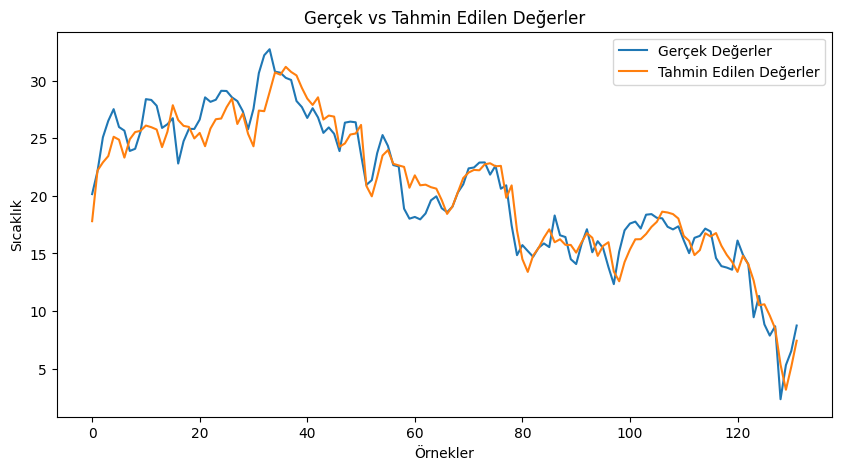
\includegraphics[width=\textwidth,height=\textheight,keepaspectratio]{GVST değerler.png}
  	\caption{Gerçek ve Tahmin Edilen Değerler Grafiği}
  		\vspace{0.7cm}
  \end{figure}
\newpage
\item {\bf\fontsize{12pt}{14pt}\selectfont Tahmin Çıktısı }\newline\newline
Modelin önümüzdeki dört gün için tahmin ettiği hava durumu verileri tablo şeklinde sunulur\cite{plotly_table}.
\begin{figure}[h]
  	
  	\vspace{0.5cm} 
  	\centering
  	 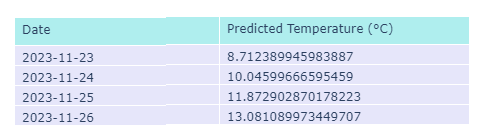
\includegraphics[width=\textwidth,height=\textheight,keepaspectratio]{newplot.png}
  	\caption{Çıktı \cite{Kizilgedik2023}}
  		\vspace{0.7cm}
  \end{figure}
\begin{table}[h]
\centering
\caption{Gerkcek Veri}
\begin{tabular}{|c|c|}

\hline
\textbf{DATE} & \textbf{TEMP} \\ \hline
2023-11-23 & 8.7 \\ \hline
2023-11-24 & 11.7 \\ \hline
2023-11-25 & 10 \\ \hline
2023-11-26 & 6.1 \\ \hline
\end{tabular}

\label{tab:temp_data}
\end{table}













  \newpage
  \bibliographystyle{plain}
\bibliography{references}
  


  \end{enumerate}
 
\end{document}